\documentclass[a4paper]{article}
\usepackage[UTF8]{ctex}
\usepackage{geometry}
\usepackage{graphicx}
\usepackage{url}
\usepackage{multirow}
\usepackage{array}
\usepackage{booktabs}
\usepackage{url}
\usepackage{enumitem}
\usepackage{graphicx}
\usepackage{float}
\usepackage{amssymb}
\usepackage{amsmath}
\usepackage{subfig}
\usepackage{longtable}
\usepackage{pifont}
\usepackage{color}

\allowdisplaybreaks

\geometry{a4paper, scale=0.78}

% \begin{figure}[H]
%     \centering
%     \includegraphics[width=.55\textwidth]{E.png}
%     \caption{矩阵与列向量的乘法}
%     \label{fig:my_label_1}
% \end{figure}

% \left\{
% \begin{array}{ll}
%       x+2x+z=2 & \\
%       3x+8y+z=12 & \\
%       4y+z=2
% \end{array}
% \right.

% \begin{enumerate}[itemindent = 1em, itemsep = 0.4pt, parsep=0.5pt, topsep = 0.5pt]

% \end{enumerate}

%\stackrel{a}{\longrightarrow}

%\underbrace{}_{} %下括号

%\tableofcontents %目录,并且目录页不记录页码
% \tableofcontents
% \newpage
% \setcounter{page}{1} %new page
% \clearpage

\title{Conditional Random Field}
\author{Chen Gong}
\date{20 February 2020}

\begin{document}
\maketitle
%\pagestyle{empty}
\tableofcontents
\newpage
%\pagestyle{fancy}
\setcounter{page}{1} %new page
\clearpage
\section{Introduction}
本讲主要介绍的是条件随机场(Conditional Random Field),这个东西在机器学习中,曾经有过较大的用处,在图像处理和标注问题中大放光彩。本小节的讲解,主要是CFR机器学习体系中的背景,我们为什么要研究CRF,CRF和其他的模型相比它在什么地方进行了演变,然后对CRF模型的建立和求解进行了分析,最后得出CRF适用于怎样的问题,它有怎样的优缺点等。这个过程是很流畅的,和前面讲到的概率图模型中的隐马尔可夫模型(Hidden Markov Model)和最大熵原理等都有一定的联系。细节请往下详细阅读。

\section{Background}
实际上机器学习中一类最重要的问题就是分类(classify)的问题。分类的方法可以被我们分为两类,硬分类和软分类。所谓硬分类就是输出值是离散的,比如$y\in \{0,1\}$;而软分类就是输出的是属于某一个类的概率,比如$P(y=1),P(y=0)$的概率。
\subsection{硬分类(Hard classification)}
硬分类就是输入特征,输出的离散变量,通俗的讲就是,分类器看到了一堆特征,直接告诉你这个个体属于哪一类。
\begin{enumerate}
    \item \textbf{支持向量机(Support Vector Machine)}:
{\color{red}支持向量机的思路来源是几何间隔}。模型可以被我们写为:
\begin{equation}
    \left\{
    \begin{array}{ll}
      \min \frac{1}{2} w^Tw & \\
      s.t. \ y_i(w^Tx_i+b) \leq 1, \ i=1,2,\cdots,N & \\
    \end{array}
    \right.
\end{equation}

\item \textbf{多层感知机(PLA):}{\color{red}多层感知机的思路来源是误差驱动}。模型可以被我们写成:
$$f(w) = \mathrm{sign}(w^Tx)$$

\item \textbf{线性判别分析(Linear Discriminate analysis):}{\color{red}主要采用的思想是类间大,类内小。}
\end{enumerate}
\subsection{软分类(Soft classification)}
软分类就是输入特征,输出的是每一种可能性的概率。通俗的讲就是,给定一组特征,分类器输出的是属于各个类别的概率,最后选择是属于哪一类?你自己就看着办吧,看你怎么选了。所以,软分类模型求得是一个分布就是这个原因。算法可以分为两个方面,概率判别模型和概率生成模型。这两者有什么不一样呢?

概率判别模型求的是$P(y|x)$;也就是将label根据提供的特征,学习,最后画出了一个明显或许比较明显的边界,比如SVM,Perceptron,神经网络,LR等都是这么工作的。

而概率生成模型求的是联合概率分布$P(x,y)$,然后你来了一个新的数据以后,我们通过贝叶斯公式化简,我们可以得到$P(y|x) \propto P(x,y)$,从而得到$P(y|x)$。生成模型关注结果是如何产生的,可以求出所有label的概率。它包含的信息非常的全,不仅可以用来输出label,还可以用来做很多别的事情。所以,生成模型需要非常多的数据量来保证采样到了数据本来的面目,所以速度慢。
\subsubsection{概率判别模型}
概率判别模型中,最基础的算法就是Logistics Regression,这个算法非常的简单。我们曾经在指数族分布那一章讲过,在给定数据和已知事实的情况下,指数族分布是可以使所有的结果经历等可能出现的分布,也就是满足最大熵原理。看到这,大家估计对最大熵原理有点懵逼,之前老师也只是提到了这个原理并说明了这个原理是什么,对于为什么并没有更层次的讲解。我们接下来讲解一下:

\textbf{最大熵原理:}其定义是对于概率模型,在所有可能分布的概率模型中,熵最大的模型是最好的模型,也就是令所有的结果都有可能出现。有的同学就会发出疑问,一方面我们总希望将事物的不确定性降到最低;另一方面对于不确定的事物我们又认为保留最大的不确定性是最好的选择。这样做不会精神分裂吗?我觉得可以这样来思考,对于我们知道的部分,我们要尽可能去靠近它;对于我们不知道的部分,我们要保持它的结果等可能的出现的可能性,就是最大限度的保留不确定性。而等可能性就是由熵最大来刻画的。俗话所说:“知之为知之,不知为不知,是知也。”

这里我们只给出最大熵原理一些直观的概念,并没有对其进行深入的理论研究,这并不是我们这节的重点。在这里我们描述的目的,是想说明\textbf{Logistics Regression是最大熵原理(Maximum Entropy Model)的一个特例,使用的是最大Entropy的思想。}

小伙伴们可能在这里有点懵逼,我来简要描述一下:

首先我们介绍一下最大熵原理的求解结果,这里的推导,有兴趣的同学自己去看,我这里只写结论。实际上指数族分布那一章就推导过了,结果就是指数族分布。
\begin{equation}
    P_w(y|x) = \frac{\exp (\sum_{i=1}^n w_if_i(x,y))}{\sum_y \exp \left( \sum_{i=1}^n w_if_i(x,y) \right)}
\end{equation}

写到了这里不知道大家有没有发现,这个最大熵原理最后的求解结果和Softmax函数是一毛一样的,是不是终于知道Softmax的作用了?Softmax本来就是用来解决多分类问题的,而Logistics Regressio只是一个二分问题,所以说,LR模型本质上是最大熵模型的一个特例,下面给出详细的证明过程:
\begin{itemize}
    \item 对于给定数据集,$X=\{ x_1,x_2,\cdots,x_n \}^T$,我们构建如下图所示的特征函数:
    \begin{equation}
    f_i(x,y) = 
    \left\{
    \begin{array}{ll}
      x_i & y=1 \\
      0 & y=0 \\
    \end{array}
    \right.
    \end{equation}
    \item 根据最大熵的求解模型为:
    \begin{equation}
    \begin{split}
         \sum_y \exp \left( \sum_{i=1}^n w_if_i(x,y) \right) = & 
        \exp \left( \sum_{i=1}^n w_if_i(x,y=0) \right) + \exp \left( \sum_{i=1}^n w_if_i(x,y=1) \right) \\
        & = 1+\exp(WX)
    \end{split}
    \end{equation}
    而根据公式(2);我们可以简单的计算出后面的结果。
    \item 当$y=1$时,可得:
    \begin{equation}
        P_w(y=1|x) = \frac{\exp(WX)}{1+\exp(WX)}
    \end{equation}
    \item 当$y=0$时,可得:
    \begin{equation}
        P_w(y=1|x) = \frac{1}{1+\exp(WX)}
    \end{equation}
\end{itemize}

所以,我们可以看到LR模型,实际上就是最大熵模型的一种特殊情况。而LR模型实际上是一种Log Linear Model,为什么这么说?实际上,我们可以知道,最大熵模型的结果就是指数族分布,详情请见指数族分布。那么:
$$
\log P(x) = \log \exp (\eta^Tf(x)) = \eta^Tf(x)
$$
就是一个线性模型,所以叫Log Linear Model。实际上看到这里,大家应该已经对深度学习中的一些设定有感觉了,不是凭空来的是有理论基础的。

最后,我们对最大熵原理做一个小结,我们的CRF中将会用到这个知识。\textbf{在给定已知事实的分析下,能够令熵达到最大的分布是指数族分布。而在给定均值,方差的情况下,Gaussian Distribution的熵最大,也就是最随机,最具等可能性。}

\subsubsection{概率生成模型}
\noindent \textbf{Naive Bayes算法:}概率生成模型的主要基础算法是Naive Bayes算法,贝叶斯算法主要是要求满足贝叶斯假设:
$$
P(X|Y=1/0) = \prod_{i=1}^P P(x_i|Y=1/0)
$$
Bayes假设的概率图模型如下所示,根据概率图模型的D-Separation原则,这是一个Tail To Tail的模型在中间值给定的情况下,其他的节点之间都是相互独立的。
\begin{figure}[H]
    \centering
    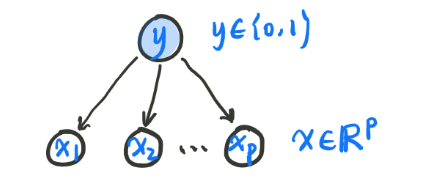
\includegraphics[width=.45\textwidth]{微信图片_20191104091918.png}
    \caption{条件独立性假设}
    \label{fig:my_label_1}
\end{figure}
\noindent 我们可以将其定义为$x_i\perp x_j|y\ (i \neq j)$。根据贝叶斯公式可以得:
\begin{equation}
    p(y|x)=\frac{p(x|y)p(y)}{p(x)}=\frac{p(x,y)}{p(x)}\propto p(x,y)
\end{equation}

而做条件独立性假设的最终目的,是为了简化运算。因为对于一个数据序列$x=(x_1,x_2,\cdots,x_p)$。如果$x_i$和$x_j$之间有关系的话,这个计算难度可能会变得很难,所以就假设各个变量之间是相互独立的。但是为了简化计算,这个假设太强了,显然有点不合理,没有充分利用数据之间的分布。

而我们将$y(0/1\rightarrow \mathrm{Seq})$就得到了Hidden Markov Model (HMM),这是我们得到HMM的第一种思路。

~\\
\noindent \textbf{高斯混合模型(Gaussian Mixture Model):}
高斯混合模型的概率图可以被我们描述为如下形式:
\begin{figure}[H]
    \centering
    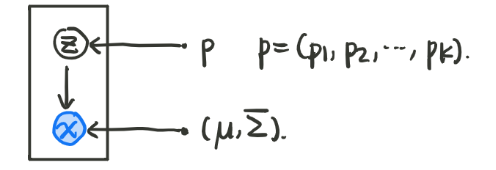
\includegraphics[width=.45\textwidth]{微信图片_20191223234640.png}
    \caption{GMM的概率图表达形式}
    \label{fig:my_label_1}
\end{figure}
我们根据一个离散的随机变量$Z$来选择是选取那个高斯分布,利用这个高斯分布$\mathcal{N}(\mu,\Sigma)$来采样得到我们想要的样本点。而且,离散随机变量$Z$符合一个离散分布$p = (p_1,p_2,\cdots,p_k)$。也就是$P(X|Z)\sim \mathcal{N}(\mu,\Sigma)$,而在此基础上加上时间的影响就构成了Hidden Markov Model,这是HMM的第二种引出方式。

~\\
\textbf{隐马尔可夫模型(Hidden Markov Model):}这个在我们之间的章节中有非常详细的描述,这里不再做过多的阐述,有兴趣的同学可以去仔细的观看。HMM中有两条非常重要的假设,齐次马尔可夫假设和观测独立假设,我们的计算基本都是基于这两个假设来的。

Hidden Markov Model的概率图模型如下所示:
\begin{figure}[H]
    \centering
    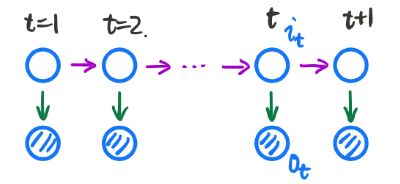
\includegraphics[width=.45\textwidth]{微信图片_20200107213811.png}
    \caption{Hidden Markov Model拓扑结构图}
    \label{fig:my_label_1}
\end{figure}
其中,$x_1$为observe data,$y_1$为lactent data,模型整体描述为$\lambda = (\pi,\mathcal{A},\mathcal{B})$。而实际上,我们还是感觉两个假设不太合理,限制了对数据集的利用,只是因为需要简化计算,所有没办法。但是,后来研究人员还是想消除假设,从而释放数据中更多的信息。

~\\
\textbf{最大熵马尔可夫模型(Maximum Entropy Markov Model):}
这里我们只对MEMM模型做一些简单的描述,尽量上直观的去解释。

MEMM是最大熵模型和HMM的结合体,它是一个判别模型。这里强调一下,它和HMM的主要区别是:\textbf{打破了HMM的观测独立假设。}这里我们后面会详细的描述。MEMM在建模过程中用到了公式(2)中,最大熵模型的求解结果,主体还是用的HMM的结构,所以,被称为最大熵马尔可夫模型。

MEMM的做法就是把输入分成两部分,1. 是所有的的$x_{1:T}$对$y$的输入;2. 单独一个上一个状态$x_{t-1}$,local输入。有的同学可能会觉得有点奇怪,$x_{1:T}$中不就包括了$x_{t-1}$,对的实际上很多时候都只看$x_{1:T}$,这样分开说是为了便于理解在HMM上的改进。MEMM的概率图模型如下所示:
\begin{figure}[H]
    \centering
    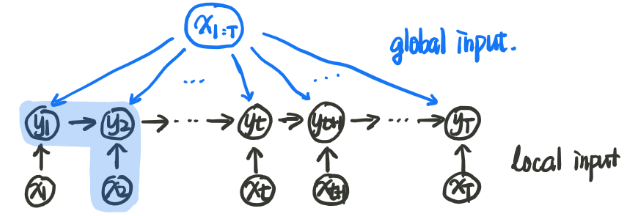
\includegraphics[width=.65\textwidth]{微信图片_20200221182717.png}
    \caption{MEMM的概率图模型}
    \label{fig:my_label_1}
\end{figure}

这小节的主要目的是引出我们为什么得到了Conditional Random Field。MEMM的细节不做过多解释。MEMM的诞生1. 首先将HMM中的观测独立假设给丢掉了,这样可以更多的使用原始数据中的信息;2. 而且,我们关注的问题从求解联合概率分布$P(X,Y)$转换成了求解$P(Y|X)$。在标注问题中并不需要计算那么多,求解$P(Y|X)$就够了。

~\\
\noindent \textbf{条件随机场(Conditional Random Field)}
虽然,MEMM有了很大的改进,但是在历史的舞台了,MEMM并没有大放光彩,这是为什么呢?由于MEMM有一个致命的问题叫做“Label Bias Problem”,这个问题主要产生的原因是局部归一化,这个问题还挺难的,这里简要的介绍一下,有兴趣的同学去看John Latterfy的相关文献。

我们简单介绍一下,看到图四中的阴影部分:为$P(y_2|y_1,x_2)$局部是一个条件概率。为了让最后的结果都是一个概率分布,我们必须要做归一化处理:
$$
\frac{\phi(y_1,x_1,y_2)}{\sum \phi (y_1,\cdots)}
$$
这就是局部归一化的意思,至于会出现怎样的原因,这里没说,后面再做出详细的分析。这个原因是因为有向图的原因造成的,那么我们把有向图变成无向图不就可以解决这个问题了,于是条件随机场算法就诞生了。

\subsection{小结}
本小节我们从机器学习的整个框架中讨论了条件随机场是怎么来的,希望对同学们有一定的启发。判别模型和生成模型的概念还是挺重要的,搞懂之后,理解很多算法会有不一样的感受。

\section{HMM VS MEMM}
这节主要介绍演变过程。话不多说,首先介绍的是HMM。
\subsection{Hidden Markov Model}
HMM可以由Naive Bayes和Gaussian Mixture Model演变而来,是一种典型的生成模型。它的概率图模型如下所示:
\begin{figure}[H]
    \centering
    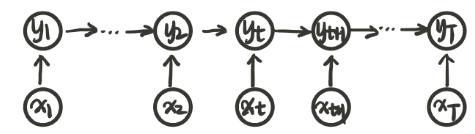
\includegraphics[width=.6\textwidth]{微信图片_20200221204618.png}
    \caption{HMM的概率图模型}
    \label{fig:my_label_1}
\end{figure}
\textbf{{\color{red}这里$x$与$y$之间的箭头画反了方向}},读者阅读的时候注意一下。模型描述为$\lambda = (\pi,\mathcal{A},\mathcal{B})$。两个假设,齐次马尔可夫假设和观测独立假设。
\begin{itemize}
    \item \textbf{齐次一阶Markov假设:}一阶:$P(y_t|y_{1:t-1})=P(y_t|y_{t-1})$;齐次:$P(y_t|y_{t-1})$与时间无关。
    \item \textbf{观测独立假设:}$P(x_t|y_{1:t},x_{1:t-1})=P(x_t|y_t)$,大家想想观测独立假设为什么会成立?这实际和Naive Bayes中提到的概率图的D-Separation有异曲同工之处。因为$y_{t-1}\rightarrow y_t \rightarrow x_{t}$是一个head to head结构,在$y_t$被观测的情况下$y_{t-1}$和$x_t$之间是独立的。
    \item \textbf{建模对象}:是$P(X,Y|\lambda)$,它要求的是一个联合概率分布。这是一个生成模型,在HMM的Evaluating问题中,需要求的是$P(X|\lambda)$,采用的大致思路都是$P(X|\lambda) = \sum_YP(X,Y|\lambda)$。经过大致的推导可以得出:
    \begin{equation}
        \begin{split}
            P(X,Y|\lambda) =  \prod_{t=1}^T P(x_t,y_t|\lambda)
            = \prod_{t=1}^T P(y_t|y_{t-1},\lambda)\cdot P(x_t|y_t,\lambda)
        \end{split}
    \end{equation}
    但是,这个实际上并不会求,算法的复杂度是$\mathcal{O}(T^N)$的,所有才有了后来的Forward和Backward算法这些。
\end{itemize}

其实观测独立假设,并没有什么道理可讲的。从NB$\rightarrow$HMM是一样的。NB中假设所有的样本之间相互独立,采用的是Tail to Tail的概率图模型,这样都是为了使计算变得简单而已。实际上这两种假设都是非必须的,都是为了计算,有它们反而破坏了原始数据分布的完整性。
\subsection{Maximum Entropy Markov Model}
MEMM模型的概率图如下图所示:
\begin{figure}[H]
    \centering
    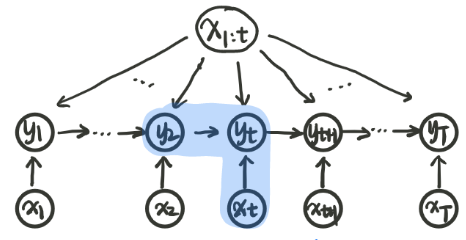
\includegraphics[width=.5\textwidth]{微信图片_20200221213227.png}
    \caption{MEMM的概率图模型}
    \label{fig:my_label_1}
\end{figure}
在MEMM中打破了观测独立假设,它是如何做到了呢?

大家注意观察,在MEMM中的$y$和$x$之间的箭头是相反的。那么,阴影部分就变成了$y_{t-1} \rightarrow y_t \leftarrow x_{t}$。这种结构是典型的Head to Tail结构,根据D-Separation原则,在$y_t$被观察到的情况下,$y_{t-1}$和$x_{t}$之间反而是有关系的。所以,它成功的打破了观测独立假设。

MEMM不再是一个生成式模型而是一个判别式模型。

根据上面的描述我们发现,$y_t$和$y_{t-1},x_t,x_{1:T}$之间都是有关系的。所以我们可以得到:
\begin{equation}
    P(Y|X,\lambda) = \prod_{t=1}^T P(y_t|x_t,y_{t-1},\lambda) = \prod_{t=1}^T P(y_t|x_{1:T},y_{t-1},\lambda)
\end{equation}
所以,我们可以很清楚的看到可以是一个全量的输出,实际上只写上面就是OK的。在概率图模型中,只画上一半就可以了。而为了和HMM作较,我们这样写可以看出分成了两个部分,看到了Global和Local的影响。

\subsection{小结}
MEMM比HMM有两个根有优势的地方:

1. 将生成模型变成了判别模型,不是说生成模型不够好,实际上是各具优点的。这里好的原因是,对于链式结构,我们主要处理的是标注问题,只要对条件建模就行了,没必要算那么多。至于为什么将生成模型变成了判别模型呢?这里老师没有讲,我来说说自己的观点。

\textbf{在HMM中,根据概率图我们得到的解是$P(x_t|y_t)$这种形式的,我们想要求的是$p(y_t|x_t)$这种形式的。对于$P(Y|X)$型的,我们只能利用$P(Y|X)P(X) = P(X,Y)$,然后来求解$P(X|Y)$,所以是生成模型。而,MEMM中直接就是$P(y_t|\cdots)$所以是判别模型。}有同学有更好的理解,欢迎留言。

2. 打破了观测独立假设,物理上更有优势了,可以尽可能多的利用到原始数据分布之间的信息。

\section{MEMM VS CRF}
MEMM的概率图模型在之前我们就展示过了,为了方便大家对下面内容的理解。这里再放一下:
\begin{figure}[H]
    \centering
    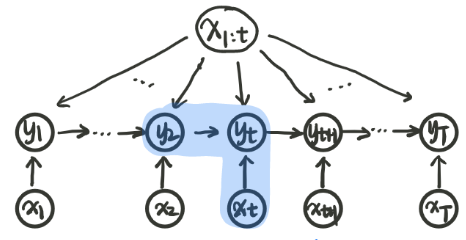
\includegraphics[width=.5\textwidth]{微信图片_20200221213227.png}
    \caption{MEMM的概率图模型}
    \label{fig:my_label_1}
\end{figure}
优点(和HMM想比):1. 判别式模型,有利于标注问题的Decoding;2. 打破了观察独立假设。

模型为:$P(Y|X,\lambda)=\prod_t P(y_t|y_{t-1},x_{1:T},x_t,\lambda)=\prod_t P(y_t|y_{t-1},x_{1:T},\lambda)$。MEMM是有向图,条件概率的条件都是在图中根据因果关系可以得出来的。

实际上我们之前说到,HMM中的两个假设实际上,并不是很合理。而在HMM中,我们通过了将$x$和$y$之间的箭头改变的方法,成功的去除了观测独立假设。而接下来MEMM到CRF的演变,实际上是解决了齐次马尔可夫假设。

在MEMM中,它的概率图模型中带来了一个重大的缺陷就是Label Bias Problem。通过将这个问题解决,我们正好就解除了齐次马尔可夫假设的限制。下面我们来描述这个问题:

\subsection{MEMM中的Label Bias Problem}
\subsubsection{Label Bias Problem定性分析}
我们的定性的来看一下Label Bias Problem。实际上图7中的阴影部分可以被我们看成是一个Logistics Regression,为什么可以这样看?实际上是因为在MEMM的建模中,我们使用的是最大熵模型,而Logistics Regression就是最大熵模型的一个特例,这里可以将一个局部看成是一个Logistics Regression。

假设我们将这个局部看成是一个系统的话,我可以将$y$看成是系统内部的状态,$y_{t-1}\rightarrow y_{t}$的转移符合一个概率分布,而$x_t$被我们看成是外界的输入。那么这个局部会不会产生怎样的问题呢?我们现在把这个局部产生的效果记为“mass score”,那么这个名词它究竟是来自哪呢?如果针对一组连续变量,它的概率密度函数就是Probability Density Function (PDF);如果是连续的变量呢?则被称之为Probability Mass Function (PMF),这个mass就是来自这,特征离散变量。这个mass score,可以看成是一个函数,就是系统从$t-1$时刻到$t$时刻转移的一个得分,这个得分就是一个概率分布。这是一个函数,它和$y_{t-1}$,$y_t$和$x_t$都是有关系的。并且状态之间的转移都是具有定的能量的,而我们的问题出在哪呢?就是这个得分函数被归一化了。为什么要归一化?因为这三个小单体形成的一个局部,实际上是一个\textbf{概率分布},概率分布就一定要归一化。

这个归一化是会带来一系列问题的,我们直观上来理解一下,他会带来的问题。如果把这个链条看成是一根长的绳子,我们在t这个点抖动一下这根绳子,肯定会对后续的绳子$t+1,t+2,\cdots$都造成影响,但是如果在中间进行归一化,就相当于在某个点把绳子的结构粗细发生了变化。那么这个波就无法正常的影响到后面的绳子了,破坏了这个波能量的传递连贯性。这是一个比较形象的例子,我们下面引入John Lafferty论文中例子来给出一个形象的解释。

\subsubsection{John Lafferty论文中例子}
归一化的不恰当会带来一些问题,但是论文中写的很简单,大多数同学看着会一脸懵逼,在这里我们做出了比较详细的讲解。例子的概率图模型如下所示:
\begin{figure}[H]
    \centering
    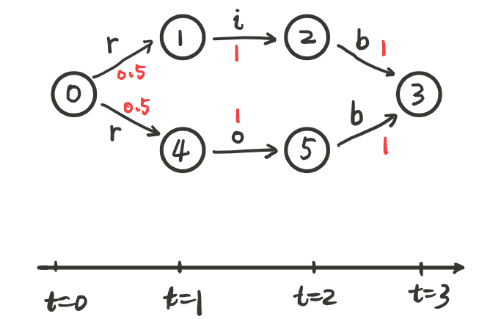
\includegraphics[width=.35\textwidth]{微信图片_20200222210750.png}
    \caption{John Lafferty论文中例子}
    \label{fig:my_label_1}
\end{figure}
在此例中,我们将$0-1-2-3-4-5$这些看成是tag标准,将$r,i,b$看成是观测。

1. 假设$t=1$时刻,我们观察到的是0,$0$时刻在观测到$r$的情况下转移到$1$和$4$状态的转移概率都一样。

2. 因为局部归一化的过程,我们发现从1到2的状态转移概率变成了1,和输入的变量根本就没有关系了。这里的路只有一条,我们假设$1\rightarrow y_{t-1}$,$2\rightarrow y_{t}$,$i\rightarrow r_t$,我们看到这里输入根本就不起作用了,不care输入是什么,概率都是1,这就是问题的所在:
\begin{equation*}
    \begin{split}
        & P(2|1,i)=1=P(2|1) \\
        & P(5|4,o)=1=P(5|4)
    \end{split}
\end{equation*}
可以看出从$1$转移到$2$根本没有关注observation。

3. 我们这里举一个例子,“小明爱中国!”,这里“小明”是名词,“爱”是动词,正常的思路是看到“中国”然后标名词。而局部归一化就是不考虑observation,不看中国了,直接根据历史的结果得出中国的词性,这显然会出问题。

4. 我们知道图模型的参数结构都是通过训练得来的。我们假设有四个样本,3个rob,1个rib。

在training的过程中,我们可以得到$P(1|0,r)=0.25$,$P(4|0,r)=0.75$。

我们使用Viterbi算法进行Decoding操作,也就是在观察序列的情况下求最大隐状态序列,$Y=(y_1,y_2,y_3)$。
\begin{equation*}
    \hat{y} = \arg\max_{y_1,y_2,y_3}(y_1,y_2,y_3|rib) = \max \{ 0.75\times 1 \times 1, 0.25\times 1 \times 1, \}
\end{equation*}
这样我们求出的,在观测为rib的情况下,隐状态链反而为$0-4-5-3$,这显然是不合适的,没有关注输入变量的影响,之间就做出了判断。

~\\
\qquad 我们举的例子是一个极端,这里的局部分布的熵直接等于0了。在这个例子中局部归一化使得系统不关注observation直接做出了判断。这是因为概率分布的熵太低了,直接等于0了,不再关注输入是什么。熵太低了就会影响模型的泛函能力,对于无法确定的信息过多的使用历史信息。\textbf{较好的模型应该,对于知道的部分,要尽可能去靠近它;对于不知道的部分,要保持它的结果等可能的出现的可能性,就是最大限度的保留不确定性,也就等价于模型的熵越大。}

在我们研究的这个问题中,可以描述为{\color{red}\textbf{Conditional Distribution with a low entropy take less notice of observation}}。

\subsection{小结}
MEMM的致命缺陷就是局部归一化,由于这个特性,会导致模型不care observation的内容来直接得到结果。其实,就是局部分布的熵太低了,对于不确定的部分,没有保留更多的可能性。

那么,打破的方法就是将各个$y$节点之间的连接从有向图变成无向图。无向图局部就不是一个分布了,就不需要进行局部归一化,而是进行全局归一化了,整条链是一个分布,这里后面后详细讲解。从而提高模型之间的熵,而有向图变成了无向图就自然打破了齐次马尔可夫假设。这是我们得到了一个chain-structure CRF,所有的$Y$节点就构成了一个随机场。

我们看到从HMM$\rightarrow$MEMM$\rightarrow$CRF,这两步过程就是先破坏了观测独立假设,再破坏了齐次马尔可夫假设。去掉了这两个不太好的假设,使原始数据得到了很好的利用。

\section{CRF概率密度函数的参数形式}
前面我们花了大量的功夫来将CRF是如何演变来的,讲述了从HMM-MEMM-CRF的演化过程,理性的讲述了CRF图结构的合理性。所谓条件随机场,我们分成两个部分来进行解释:条件指的是,条件概率;随机场指的是,$y$节点连接而成的无向图模型,称之为Markov Field。CRF的概率图模型如下所示:
\begin{figure}[H]
    \centering
    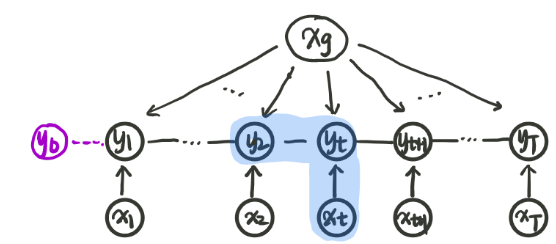
\includegraphics[width=.55\textwidth]{微信图片_20200223000157.png}
    \caption{CRF的概率图模型}
    \label{fig:my_label_1}
\end{figure}

\subsection{势函数化简}
我们想要得出\textbf{$P(Y|X)$}的形式,很可惜在无向图中,我们并不能根据因果关系直接写出来。我们之间讲到过无向图的分解方法,这里再重申一下团的概念,\textbf{一个图中所有节点之间都相互相连称之为团}。对于Markov Random Field做因子分解,对于$x\in \mathbb{R}^p$,我们可以令:
$$
P(X) = \frac{1}{Z} \prod_{i=1}^k \phi_i(x_{c_i}) = \frac{1}{Z} \prod_{i=1}^k \exp \{ -E_i(x_{c_i}) \}
$$
这里的$K$表示有$k$个最大团,$c_i$指的是第$i$个最大团,而$\phi_i(x_{c_i})$表示第$i$个最大团的势函数。$\phi_i(x_{c_i})$:势函数,必须为正。这里的概念都是来自于统计物理学和热力学的过程。因为,势函数必定为正,我们可以将势函数表达为$\phi_i(x_{c_i}) = \exp\{ -E_i(x_{c_i}) \}$。其中,$E_i(x_{c_i})$称为Energy function。实际上用这种形式表达的$p(x)$,为Gibbs Distribution,或者又被称之为Boltzman Distribution。为了进一步简化,我们令$-E_i(x_{c_i})=F_i(x_{c_i})$,所以就得到了最终的形式:
\begin{equation}
    P(X) = \frac{1}{Z} \prod_{i=1}^k \exp \{ F_i(x_{c_i}) \}
\end{equation}

\subsection{CRF概率参数结构}
如果不加说明,我们认为CRF为线性链。
\begin{figure}[H]
    \centering
    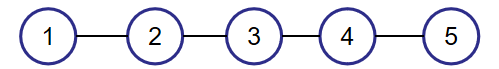
\includegraphics[width=.45\textwidth]{微信图片_20200223114928.png}
    \caption{线性链模型}
    \label{fig:my_label_1}
\end{figure}
我们可以看到在线性链中,每两个相邻的节点之间形成了一个团,而且总有团的机构都是一样的,图10所例的线性链可以被我们分成4个团。每个团都和$y_t$,$y_{t-1}$和$x_{1:T}$有关系,所以,
\begin{equation}
    \begin{split}
        P(X) 
        = & \frac{1}{Z} \prod_{i=1}^k \exp \{ F_i(x_{c_i}) \} = \frac{1}{Z} \exp \sum_{i=1}^{T-1} F_t(y_{t-1},y_t,x_{1:T})
    \end{split}
\end{equation}
这个公式的转换,首先将连乘写到指数函数里变成了连加,又因为线性链所有团的结构都是一样的。所以相当于从第1个加到第$T-1$个。由于线性链中所有团的结构都是一样的,我们只考虑其中的一个团结构。那么,下一步的目标则是考虑,$F_t(y_{t-1},y_t,x_{1:T})$怎么表示?

这个结构的得来实际上有一定的intuitive,我们将它分成两部分,状态函数和转移函数。状态函数包括$y_t$时刻和$y_{t-1}$时刻和$x_{1:T}$之间的影响,转移函数包括$y_t,y_{t-1}$时刻共同和$x_{1:T}$之间的影响。公式表达如下所示:
\begin{equation}
    F_t(y_{t-1},y_t,x_{1:T}) = \underbrace{\triangle_{y_{t-1},x_{1:T}}+ \triangle_{y_{t},x_{1:T}}}_{\mathrm{State\ Function}} + \underbrace{ \triangle_{y_{t-1},y_t,x_{1:T}}}_{\mathrm{Transfer\ Function}}
\end{equation}
这里再次提醒一下,我们代入到标注问题中,$x_{1:T}$为“小明是中国人。”这是我们观测到的值,$y_{t-1}$和$y_t$代表隐变量为词语的词性,名词,动词和形容词等。状态函数中$y_t$对$t$时刻的影响已经包含了$y_{t-1}$时刻的影响,我们没有必要再计算两遍,所以在状态函数中我们可以忽略掉$y_{t-1}$。所以,最终结果为;
\begin{equation}
    F_t(y_{t-1},y_t,x_{1:T}) = \triangle_{y_{t},x_{1:T}} + \triangle_{y_{t-1},y_t,x_{1:T}}
\end{equation}
我们用一个函数来表达$\triangle_{y_{t},x_{1:T}}$:
\begin{equation}
    \triangle_{y_{t},x_{1:T}} = \sum_{l=1}^L \eta_l g_l(y_t,x_{1:T})
\end{equation}
其中$f_k$为特征函数,指示函数,满足某个状态为1,比如:
$$
f_k(y_{t-1}=\mathrm{noun},y_t=\mathrm{verb},x_{1:T})=1
$$
$$
f_k(y_{t-1}=\mathrm{noun},y_t=\mathrm{auxiliary},x_{1:T})=0
$$
而$\lambda_k$则是我们需要学习的参数,利用数据通过Learning来得到。同样,我们可以用类似的思路来定义$\triangle_{y_{t-1},y_t,x_{1:T}}$:
$$
\triangle_{y_{t-1},y_t,x_{1:T}} = \sum_{k=1}^K \lambda_k f_k(y_{t-1},y_t,x_{1:T})
$$
这里的$f_k$和$g_l$都是给定的特征函数,$\lambda_k$和$\eta_l$都是需要学习的参数。所以,我们最后就得到了CRF条件概率的表达形式为:
\begin{equation}
    P(Y|X) = \frac{1}{Z} \exp \left\{ \sum_{t=1}^T \left[ \sum_{k=1}^K \lambda_k f_k(y_{t-1},y_t,x_{1:T}) + \sum_{l=1}^L \eta_l g_l(y_t,x_{1:T}) \right] \right\}
\end{equation}
这就是CRF的概率密度函数,实际上这个得出的过程是比较Intuitive的,可能大家有点不太好理解。那么,我们来做一个类比,对于学习机器的同学来说,肯定对神经网络非常的熟悉。对于图像识别问题,我们输入一张图片,通过一个网络,得到一个结果。对于这个网络,我们选择怎样的网络结构,是前馈神经网络,CNN还是RNN,什么样的激活函数,和怎样的激活函数都是一个结构,然后根据我们的结果使用梯度下降来训练得到相应的参数。实际上这里和神经网络的结构是一个的,就像神经网络为什么设置成那个样子,实际上也不能说的很明白,就是这样的结构会make sence而已。在这里也一样,我的设计出的概率密度函数形式,就是感觉符合CRF的网络结构,并且会make sence,当然小伙伴有更好的想法,也可以改进这个参数结果。得到结构后,我们就可以通过训练来求得参数了。

\subsection{小结}
在这一小节中,我们比较intuitive的得到了CRF概率密度函数的参数形式,和神经网络一样,这都是我们为了实现目的根据概率图的结构而设计出的一种会make sence的结构。结构确定之后,通过对数据的训练来求得参数,那么CRF模型就建立完成了。

\section{概率密度函数的向量形式}
上一节中,我们讲到了可以将每一个最大团分成两个部分,即为状态函数和转移函数。
\begin{equation}
    \begin{split}
        P(Y|X) = & \frac{1}{Z} \exp\sum_{t=1}^T [\triangle_{\mathrm{transfer\ function}}+\triangle_{\mathrm{state\ function}}] \\
        = & \frac{1}{Z} \exp \left\{ \sum_{t=1}^T \left[ \sum_{k=1}^K \lambda_k f_k(y_{t-1},y_t,x_{1:T}) + \sum_{l=1}^L \eta_l g_l(y_t,x_{1:T}) \right] \right\}
    \end{split}
\end{equation}
这里的K和L分别是多少呢?加入对于$y_t \in S = \{noun,verb,aux,\cdots\}$一共有$S$个状态。我们看看转移图像:
\begin{figure}[H]
    \centering
    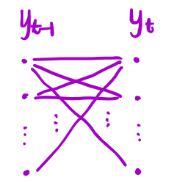
\includegraphics[width=.25\textwidth]{微信图片_20200223151838.png}
    \caption{$y_{t-1}$和$y-t$状态之间的转移}
    \label{fig:my_label_1}
\end{figure}
所以,我们看到最多有$|S|^2$种可能,所以$\mathrm{K}\leq |S|^2$。对于归一化因子$Z$而言,肯定是和$y$没有关系的,归一化因子是对$y$进行了积分的。
\subsection{概率密度函数的向量形式化简}
所以,概率模型被我们写为:
\begin{equation}
    P(Y=y|X=x) = \frac{1}{Z(x,\lambda,\eta)} \exp \left\{ \sum_{t=1}^T \left[ \sum_{k=1}^K \lambda_k f_k(y_{t-1},y_t,x_{1:T}) + \sum_{l=1}^L \eta_l g_l(y_t,x_{1:T}) \right] \right\}
\end{equation}
令:
\begin{equation}
    \lambda =
    \begin{bmatrix}
    \lambda_1 \\
    \lambda_2 \\
    \vdots \\
    \lambda_k
    \end{bmatrix}, \qquad
    \eta =
    \begin{bmatrix}
    \eta_1 \\
    \eta_2 \\
    \vdots \\
    \eta_l
    \end{bmatrix}, \qquad
    f = 
    \begin{bmatrix}
    f_1 \\
    f_2 \\
    \vdots \\
    f_k
    \end{bmatrix} = f(y_{t-1},y_t,x_{1:T}), \qquad
    g = 
    \begin{bmatrix}
    g_1 \\
    g_2 \\
    \vdots \\
    g_l
    \end{bmatrix} = g(y_t,x_{1:T})
\end{equation}
根据向量的内积方法,我们可以将$\sum_{k=1}^K \lambda_k f_k(y_{t-1},y_t,x_{1:T})$改写为$\lambda^T f(y_{t-1},y_t,x_{1:T})$,$\sum_{l=1}^L \eta_l g_l(y_t,x_{1:T})$改写为$\eta^T g(y_t,x_{1:T})$。所以,原式等于:
\begin{equation}
\begin{split}
    P(Y=y|X=x) = & \frac{1}{Z(x,\lambda,\eta)} \exp \left\{ \sum_{t=1}^T \left[ \lambda^T f(y_{t-1},y_t,x_{1:T}) + \eta^T g(y_t,x_{1:T})) \right] \right\} \\
    = & \frac{1}{Z(x,\lambda,\eta)} \exp \left\{ \left[  \lambda^T \sum_{t=1}^T f(y_{t-1},y_t,x_{1:T}) +  \eta^T\sum_{t=1}^T g(y_t,x_{1:T})) \right] \right\}
\end{split}
\end{equation}
我们现在看着还是觉得太复杂还想进行下一步化简,这里的$\lambda$和$\sum_{t=1}^T f(y_{t-1},y_t,x_{1:T})$都是$k \times 1$的向量,$\eta$和$\sum_{t=1}^T g(y_t,x_{1:T})$都是$l \times 1$的向量,相加是在同一个维度相加,并不会破坏矩阵的尺寸。所以我们可以进行合并。于是令:
\begin{equation}
    \theta = \begin{bmatrix} \lambda\\ \eta \end{bmatrix}_{(k+l)\times 1}, \qquad
    H = \begin{bmatrix} \sum_{t=1}^T f(y_{t-1},y_t,x_{1:T})\\ \sum_{t=1}^T g(y_t,x_{1:T})) \end{bmatrix}_{(k+l)\times 1}, \qquad
\end{equation}

所以,我们得到的形式为:
\begin{equation}
     P(Y=y|X=x) = \frac{1}{Z(x,\theta)} \exp \left\{ \theta^T \cdot H(y_t,y_{t-1},x_{1:T}) \right\} 
\end{equation}
$H(y_t,y_{t-1},x_{1:T})$表示$H$矩阵和$y_t,y_{t-1},x_{1:T}$有关。我们可以将$\theta^T \cdot H(y_t,y_{t-1},x_{1:T}$写成向量内积的形式,最终得到最后的形式为:
\begin{equation}
    P(Y=y|X=x) = \frac{1}{Z(x,\theta)} \exp \langle \theta,H \rangle
\end{equation}

\subsection{小结}
我们最终得到了概率密度函数的向量表达形式为:
$$
    P(Y=y|X=x) = \frac{1}{Z(x,\theta)} \exp \langle \theta,H \rangle
$$
实际上这章非常的简单,都是一些很简单的数学变形而已。我们这样做的目的是什么呢?很简单就是去掉$\sum$符号,在learning和Inference问题中,我们可能遇到大量的求导,把这个$\sum$去掉是为了简化运算,带上了$\sum$不方便进行求导运算。

\section{CRF模型要解决的问题}
上一节我们用向量形式来进行表达,为Learning和Inference问题做好了准备。所谓机器学习中需要解决的问题,大致被我们分为两类,通过learning来得到模型,并利用求得的模型对未知的数据进行Inference。
\subsection{Learning}
也就是Parameter estimation,利用数据来对模型中的参数进行求解。这么任务可以被描述为:给定一个数据集$\{ (x^{(i)},y^{(i)}) \}_{i=1}^N$,其中$x,y\in \mathbb{R}^T$都是T维的。

我们可以来举一个简单的例子,比如“小明爱中国”,这个数据的$x$由三个部分组成,分别是“小明”,“爱”和“中国”组成的,标注$y$则是“名词”,“动词”,“名词”组成的。在我们的CRF概率图中,不是一个节点是一个样本,而是所有的$y$节点合在一起才是一个样本,这里需要强调一下以防同学弄混。所有,我们最终的求解目标为:
\begin{equation}
    \hat{\theta} = \arg\max \prod_{i=1}^N P(y^{(i)}|x^{(i)})
\end{equation}

\subsection{Inference}
Inference通常可以被我们分为Marginal Probability;Conditional Probability和MAP Inference: Decoding三类问题。而CRF是判别模型,所以我们一般不谈Conditional Probability,这个一般是针对生成模型中才会用到的,因为求联合概率,我们通常是使用贝叶斯公式来进行转换的。所以,我们这里不讨论CRF的Conditional Probability的问题。

\subsection{Marginal Probability}
在概率图模型中,我们的建模对象往往都是join distribution。比如有一个建模对象为$P(X)$,$X=(x_1,x_2,\cdots,x_p)^T$。我们要求$P(x_1)$,往往都是先求$P(X)$,然后再对其他变量进行积分来求得$P(x_1)$。

举例,词性标注问题,对于$P(y_1=verb|X)$,也就是给定观察序列,求第$i$个词是动词的概率。

% \subsection{Conditional Probability}
% 对于典型的HMM问题,这是一个生成模型,假定观测变量是$X$,隐状态变量是$Y$,我们要求的就是知道观测变量$Y$后的,隐状态变量的序列,我们要求的是一个序列。即为:
% \begin{equation}
%     \hat{Y} = \arg\max_Y P(Y|X)
% \end{equation}

\subsection{MAP Inference: Decoding}
Decoding问题,也就是在给定观察序列的情况下,寻找最大概率可能出现的隐概率状态序列。求解的是:
\begin{equation}
    \hat{Y} = \arg\max_{Y=y_1,\cdots,y_t} P(Y|X)
\end{equation}

\subsection{小结}
下面我们主要针对CRF的三个问题进行求解,分别是1. Marginal Probability;2. Parameter Estimation;3. Decoding Problem。

\section{Marginal Probability Calculate}
在描述这个问题之前,先假设参数是已知的,如果参数是未知的,那么就假设参数$\theta$是一个常量。我们的求解目标是,\textbf{给定$P(Y=y|X=x)$的情况下,求$P(y_t=i|x)$的概率},这里再强调一下,每一个$\{x,y\}$都是一个时序的样本,比如一个句子,每个样本可以根据时间分成很多段。

\subsection{直接进行求解}
概率密度函数被定义为:
\begin{equation}
    P(Y=y|X=x) = \frac{1}{Z} \prod_{t=1}^T \phi_t(y_{t-1},y_t,x)
\end{equation}
实际上就等于最大团的势函数之积。我们要求某个时刻在已知所有的观察变量的情况下隐变量$y_t=i$的概率,实际上就是将$P(Y=y|X=x)$这个联合概率分布在$y$的各个维度上积分,就可以得到$y_t$时刻的条件概率了,而这里都是离散变量,那么就是求和。这个思路和想法很简单,我们来看看它怎么样?
\begin{equation}
    P(y_t=i|x) = \sum_{y_1,\cdots,y_{t-1},y_{t+1},\cdots,y_T} P(y|x) = \sum_{y_{1:t-1}} \sum_{y_{t+1:T}} \frac{1}{Z} \prod_{t'=1}^T \phi_{t'}(y_{t'-1},y_{t'},x)
\end{equation}
由于我们求的是一个概率分布,每一个$y_t \in \mathcal{S}$,我们一共要对$T-1$个$y$进行积分,每一个$y$有$|S|$种可能,所以在这个求积分的过程中,算法的复杂度是$\mathcal{O}(|S|^T)$的。\textbf{大家都是学过高等数学的,如果你理解不了,这就是一个T-1重积分,T-1重积分是T-1维空间中的体积,因为所有势函数的乘积,所以每次都需要考虑概率图中所有的依赖关系,计算需要进行$|S|^T$次划分}。而在求势函数的积的过程中,需要进行$T$次运算,所以这个算法最后的复杂度是$\mathcal{O}(T\cdot|S|^T)$。这个算法的复杂度实在是太高了,我们根本就没有办法求解,这个想法确实很简单,但是很可惜是intractable的。

那么我们有没有什么办法来简化运算呢?

\subsection{Variables Elimination算法复杂度降低分析}
这个算法我们之前在HMM中是讲过的,在这个问题中我们怎么求解呢?上述直接进行求解的办法,\textbf{因为每一次积分都是对所有的势函数乘积进行积分,所以需要考虑所有的状态,算法复杂度是$\mathcal{O}(|S|^T)$,这是暴力求解的思路}。

我们发现,在对某一个时刻的变量$y_i$进行求和的时候,和很多的势函数都没有关系。比如在$t=5$时刻,求和只和势函数$\phi(y_4,y_5,x)$有关。所以,我们可以利用动态规划的思路,将连加号分解开,移到后面后具体相关的势函数联系起来,这样每次积分时只考虑和势函数相关的变量,不需要考虑所有的变量。\textbf{设$m$为单个条件概率的最大变量数量,我们化简后,只有依赖最多的这个节点会被考虑$m$次,其他的都会少于$m$次,所以算法复杂度被就降低到了$\mathcal{O}(|S|^m)$,而$m << T$。}这就是我们思路的大致来源。

\subsection{Variables Elimination算法运算过程}
由于在第$t$时刻,$y_t$的状态是已知的。所以,我们将序列从$y_t$时刻分开,分成两个部分,如下图所示:
\begin{figure}[H]
    \centering
    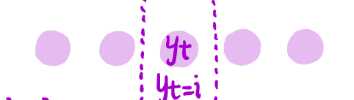
\includegraphics[width=.35\textwidth]{微信图片_20200224144010.png}
    \caption{序列分割图}
    \label{fig:my_label_1}
\end{figure}
\begin{equation}
    P(y_t=i|x) = \sum_{y_{1:t-1}} \sum_{y_{t+1:T}} \frac{1}{Z} \prod_{t'=1}^T \phi_{t'}(y_{t'-1},y_{t'},x) = \frac{1}{Z} \triangle_{\mathrm{left}}\cdot \triangle_{\mathrm{right}}
\end{equation}
其中:
\begin{equation}
\begin{split}
    & \triangle_{\mathrm{left}} = \sum_{y_{1:t-1}} \phi_1(y_0,y_1,x)\phi_2(y_1,y_2,x)\cdots\phi_{t-1}(y_{t-2},y_{t-1},x)\phi_{t}(y_{t-1},y_{t}=i,x) \\
    & \triangle_{\mathrm{right}} = \sum_{y_{t+1:T}} \phi_{t+1}(y_{t}=i,y_{t+1},x)\phi_{t+2}(y_{t+1},y_{t+2},x)\cdots\phi_{T}(y_{T-1},y_{T},x)
\end{split}
\end{equation}
下一步目标就是想怎么去拆分了,首先来看看每一个势函数究竟和哪些变量有关,示意图如下所示:
\begin{figure}[H]
    \centering
    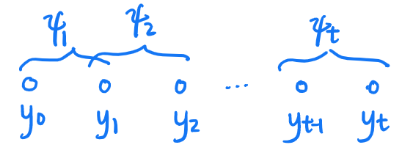
\includegraphics[width=.35\textwidth]{微信图片_20200224165315.png}
    \caption{势函数变量关系图}
    \label{fig:my_label_1}
\end{figure}
变量消除的过程就是积分的过程,我们需要将累加的变量进行分解,让求和过程只和相关的势函数进行求和,这样分解避免多个势函数混着一起积分,来减少运算过程,因为这样每次积分我们都只要考虑单个变量的依赖变量的关系。根据上图所示的,关系依赖图,我们进行如下划分:
\begin{equation}
    \begin{split}
        \triangle_{\mathrm{left}} = & \sum_{y_{1:t-1}} \phi_1(y_0,y_1,x)\phi_2(y_1,y_2,x)\cdots\phi_{t-1}(y_{t-2},y_{t-1},x)\phi_{t}(y_{t-1},y_{t}=i,x) \\
        = & \sum_{y_{t-1}} \phi_{t}(y_{t-1},y_{t}=i,x) \left( \sum_{y_{t-2}} \phi_{t-1}(y_{t-2},y_{t-1},x) \left( \cdots \left( \sum_{y_1} \phi_2(y_1,y_2,x) \left(\sum_{y_0}\phi_1(y_0,y_1,x)\right)\right) \right)\right)
    \end{split}
\end{equation}
那么这样我们手动的把所有的$\sum$连加符号,一个个的嵌入到该去的地方,计算复杂度过高的问题已经解决了。实际上写成公式(29)这样的样子就可以了。我们为了进一步简化表达作如下操作。

我们令:
$$
\alpha_t(i) = \sum_{y_{t-1}} \phi_{t}(y_{t-1},y_{t}=i,x) \left( \sum_{y_{t-2}} \phi_{t-1}(y_{t-2},y_{t-1},x) \left( \cdots \left( \sum_{y_1} \phi_2(y_1,y_2,x) \left(\sum_{y_0}\phi_1(y_0,y_1,x)\right)\right) \right)\right)
$$
$$
\alpha_{t-1}(j) =  \sum_{y_{t-2}} \phi_{t-1}(y_{t-2},y_{t-1}=j,x) \left( \cdots \left( \sum_{y_1} \phi_2(y_1,y_2,x) \left(\sum_{y_0}\phi_1(y_0,y_1,x)\right)\right) \right)
$$
那么,很显然我们就可以得出$\alpha$函数之间的表达式:
\begin{equation}
    \alpha_t(i) = \sum_{y_{t-1}} \phi_{t}(y_{t-1}=j,y_{t}=i,x) \alpha_{t-1}(j)
\end{equation}
因为,$y_{t-1}=j$,所以我们可以得到等价表达方式:
\begin{equation}
    \alpha_t(i) = \sum_{j\in S} \phi_{t}(y_{t-1}=j,y_{t}=i,x) \alpha_{t-1}(j)
\end{equation}
实际上推导到了这里就很简单了,那么$\triangle_{\mathrm{left}} = \alpha_t(i)$。按照同样的方法进行变量提取化简,我们可以得到一样的结论:
\begin{equation}
\begin{split}
    \triangle_{\mathrm{right}} = & \sum_{y_{t+1:T}} \phi_{t+1}(y_{t}=i,y_{t+1},x)\phi_{t+2}(y_{t+1},y_{t+2},x)\cdots\phi_{T}(y_{T-1},y_{T},x)\\
    = & \sum_{y_{T}} \phi_{T}(y_{T-1},y_{T},x) \left( \sum_{y_{T-1}} \phi_{T-1}(y_{T-2},y_{T-1},x) \left( \cdots \left( \sum_{y_{t+2}} \phi_2(y_{t+1},y_{t+2},x) \left(\sum_{y_{t+1}}\phi_1(y_{t}=i,y_{t+1},x)\right)\right) \right)\right) \\
    = & {\color{red} \beta_t(i)}
\end{split}
\end{equation}

所以,最终得到的最简形式为:
\begin{equation}
    P(y_t=i|x) = \frac{1}{Z} \alpha_t(i) \cdot \beta_t(i)
\end{equation}

\subsection{小结}
本小节我们探讨了给定$P(Y=y|X=x)$的情况下,求$P(y_t=i|x)$的概率,$x$和$y$都是时序序列。直接采用积分求和的方法算法复杂度为$\mathcal{O}(|S|^T)$的太高了,利用变量消元的方法,准确的分离变量和待求和的维度。\textbf{成功的将算法复杂度从$\mathcal{O}(|S|^T)$降到$\mathcal{O}(|S|^m)$,且$m$为单个条件概率的最大变量数量,$m << T$。}

\section{CRF Learning Problem}
在这个问题中,问题具体就是用极大似然估计来求CRF模型的参数,
\begin{equation}
    \hat{\theta} = \arg\max_{\theta} \prod_{i=1}^N P(y^{(i)}|x^{(i)})
\end{equation}
$N$为训练样本的数量。而$\theta$实际上包含两个部分,即为$\lambda,\eta$,所以,目标函数为:
\begin{equation}
    \hat{\lambda},\hat{\eta} = \arg\max_{\lambda,\eta} \prod_{i=1}^N P(y^{(i)}|x^{(i)})
\end{equation}
而我们,在之前求过了,
\begin{equation}
     P(Y=y|X=x) = \frac{1}{Z(x,\lambda,\eta)} \exp \left\{ \sum_{t=1}^T \left[ \lambda^T f(y_{t-1},y_t,x) + \eta^T g(y_t,x)) \right] \right\}
\end{equation}

所以:
\begin{equation}
    \begin{split}
        \hat{\lambda},\hat{\eta} = & \arg\max_{\lambda,\eta} \prod_{i=1}^N P(y^{(i)}|x^{(i)}) \\
        = & \arg\max_{\lambda,\eta} \sum_{i=1}^N \log P(y^{(i)}|x^{(i)}) \\
        = & \arg\max_{\lambda,\eta} \sum_{i=1}^N \left\{ 
        -\log Z(x^{(i)},\lambda,\eta) + \sum_{t=1}^T \left[ \lambda^T f(y_{t-1}^{(i)},y_t^{(i)},x) + \eta^T g(y_t^{(i)},x^{(i)})) \right]
        \right\} \\
        = & \arg\max_{\lambda,\eta} L(\lambda,\eta,x^{(i)}) 
    \end{split}
\end{equation}
\subsection{梯度上升法求解极大似然解}
\begin{equation}
    \nabla_\lambda L = \sum_{i=1}^N \left\{ \sum_{t=1}^Tf(y_{t-1}^{(i)},y_t^{(i)},x^{(i)}) - \nabla_\lambda  \log Z(x^{(i)},\lambda,\eta) \right\}
\end{equation}
现在问题就是$\nabla_\lambda  \log Z(x^{(i)},\lambda,\eta)$怎么来求?注意观察公式(36),$P(Y=y|X=x)$实际上是一个指数族分布。而$Z(x^{(i)},\lambda,\eta)$就是log partition function。我们在指数族分布的第三部分曾经推导出,log partition function的导数为充分统计量的均值。所以,$\nabla_\lambda  \log Z(x^{(i)},\lambda,\eta)$我们可以直接写出来的。
$$
    \mathbb{E}\left[ \sum_{i=1}^T f(y_{t-1},y_t,x^{(i)}) \right]
$$
注意这里的$y$是自变量而不是样本,所以:
\begin{equation}
    \begin{split}
       \mathbb{E}\left[ \sum_{i=1}^T f(y_{t-1},y_t,x^{(i)}) \right] = & \sum_y P(y|x^{(i)}) \cdot  \sum_{i=1}^T f(y_{t-1},y_t,x^{(i)}) \\
       = & \sum_{i=1}^T \left( \sum_y P(y|x^{(i)}) \cdot f(y_{t-1},y_t,x^{(i)})  \right)
    \end{split}
\end{equation}
因为在$f(y_{t-1},y_t,x^{(i)})$中,我们是知道具体的值的。所以,我们把其他维度的$y$都通过求和消掉。那么:
\begin{equation}
    \begin{split}
        \sum_{i=1}^T \left( \sum_y P(y|x^{(i)}) \cdot f(y_{t-1},y_t,x^{(i)})  \right) 
        = & \sum_{i=1}^T \left( \sum_{y_{1:t-2}} \sum_{y_{t-1}} \sum_{y_t} \sum_{y_{t+1:T}} P(y|x^{(i)}) \cdot f(y_{t-1},y_t,x^{(i)})  \right) \\
        = & \sum_{i=1}^T \sum_{y_{t-1}} \sum_{y_t} \left( {\color{red}\sum_{y_{1:t-2}} \sum_{y_{t+1:T}} P(y|x^{(i)})} \cdot f(y_{t-1},y_t,x^{(i)})  \right) \\
        = & \sum_{i=1}^T \sum_{y_{t-1}} \sum_{y_t} \left( {\color{red} P(y_{t-1},y_t|x^{(i)})} \cdot f(y_{t-1},y_t,x^{(i)})  \right)\\
    \end{split}
\end{equation}
那么,我们的下一步思路就是如何求解$ P(y_{t-1},y_t|x^{(i)}) $。这实际上就是一个求解边缘概率的问题。这其中$y_{t-1},y_t$都是已知的。
\begin{equation}
    \begin{split}
        P(y_{t-1}=j,y_t=i|x^{(i)}) = & \sum_{y_{1:t-2}} \sum_{t+1:T} \prod_{t'=1}^T \phi_{t'}(y_{t'-1},y_{t'},x) \\
        = & \frac{1}{Z} \triangle_{\mathrm{left}}\cdot \phi(y_t,y_{t-1},x) \cdot \triangle_{\mathrm{right}} \\
        = & \frac{1}{Z} \alpha_{t-1}(j) \cdot \phi(y_t=i,y_{t-1}=j,x) \cdot \beta_{t}(i) \\
        = & {\color{red} A(y_{t-1},y_t) }
    \end{split}
\end{equation}
所以,最后我们得到的结论为:
\begin{equation}
    \begin{split}
        \nabla_\lambda L = \sum_{i=1}^N \sum_{t=1}^T \left[ f(y_{t-1}^{(i)},y_{t}^{(i)},x^{(i)}) - \sum_{y_{t-1}}\sum_{y_t}A(y_{t-1},y_t) f(y_{t-1},y_{t},x) \right]
    \end{split}
\end{equation}
其中,$y_{t}^{(i)}$为样本,$y_{t}$为自变量。那我们用类似的方法同样可以求解出:
\begin{equation}
    \begin{split}
        \nabla_\eta L = \sum_{i=1}^N \sum_{t=1}^T \left[ f(y_{t-1}^{(i)},y_{t}^{(i)},x^{(i)}) - \sum_{y_{t-1}}\sum_{y_t}A(y_{t-1},y_t) g(y_{t},x) \right]
    \end{split}
\end{equation}
最终,梯度上升算法将被我们总结为:
\begin{equation}
\left\{
\begin{array}{ll}
      \lambda^{t+1} = \lambda^{t}+\mathrm{step}\cdot \nabla_\lambda L(\lambda^{(t)},\eta^{(t)})  & \\
      \eta^{t+1} = \eta^{t}+\mathrm{step}\cdot \nabla_\eta L(\lambda^{(t)},\eta^{(t)})  & \\
\end{array}
\right.
\end{equation}
实际上,这只是一种理论上可行的求解方法。实际求解的过程中,这样做收敛速度太慢了,这里只是给出一种理论的解,还有很多类似的方法,有兴趣的同学可以深入研究。

\subsection{MAP Inference}
这个问题,仔细观察就知道和HMM中的Decoding问题是一样的。HMM和CRF没有任何区别。我们想要在已知观测序列的情况下,求隐变量序列的最大的可能状态。实际上就是使用动态规划算法,一步步求得最大的序列,也就是Viterbi算法,在Hidden Markov Model的第四节,有详细的描述,这里就不多说。

\subsection{小结}
这一节中,我们介绍了用极大似然估计算法来求CRF模型的参数。实际上计算过程都还挺普通的。有一个难点是利用\textbf{指数族函数log partition function的导数为充分统计量的均值}这个结论来进行求解。实际上这一步明白之后,还是比较简单的。而其中也遇到了求边缘概率的方法,我们用到了之前描述的本章第8节求Marginal Probability的方法。MAP Inference和HMM中的Decoding问题是一样的,使用Viterbi算法求解。

\section{Conclusion}
本章的思路实际是很流畅的,首先介绍了整个机器学习体系结构。然后,引出了概率图模型在其中的地位。从最简单的概率图模型,Naive Bayes算法,一步步的改进缺点到HMM,到MEMM,最后演化成了CRF。我个人感觉这个过程是非常重要的,很多教科书一上来就摆了一推的概率和定义,我等凡人真的头疼。非常感谢B站白板推导系列的up主。而之后就,定义了CRF的模型结构,定义完了之后就是如何使用数据来求解这个CRF模型的参数,求解出来之后就是如何用这个模型来进行inference,整个过程的思维是非常流畅和附有逻辑性的。









\end{document}
